\section{The model}
\label{sec:application:the_model}

\begin{figure}[p]
    \centering
    \begin{subfigure}{0.98\textwidth}
        \centering
        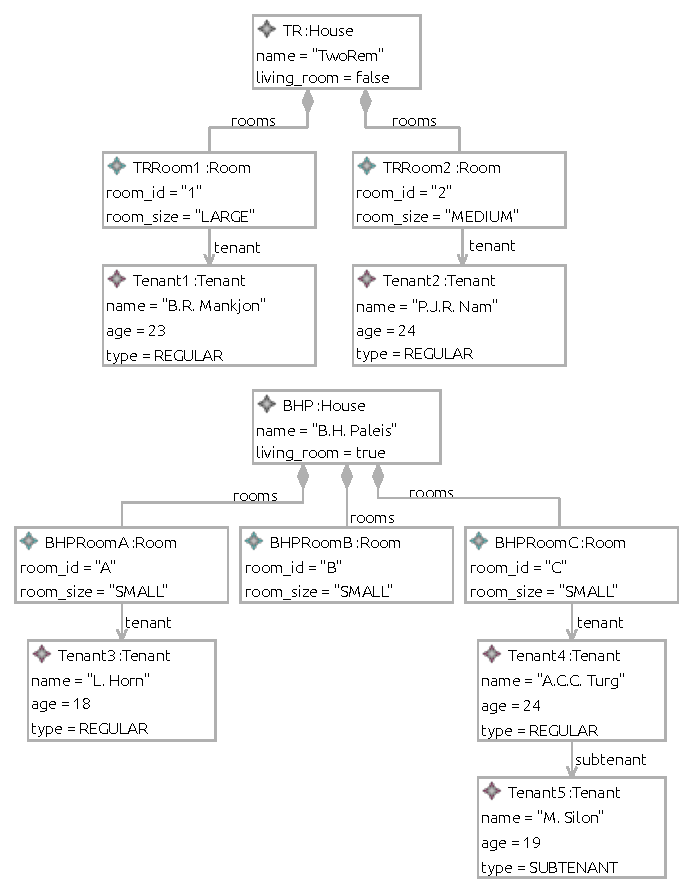
\includegraphics{images/06_application/instance_model/step15.pdf}
        \caption{Instance model}
        \label{fig:application:the_model:final_ecore_model:instance_model}
    \end{subfigure}
    \\
    \begin{subfigure}{0.98\textwidth}
        \centering
        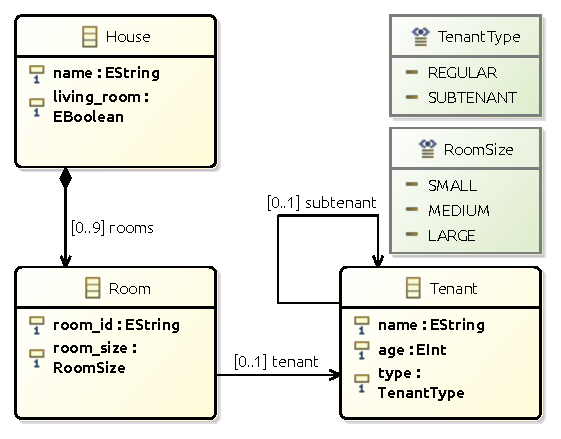
\includegraphics{images/06_application/type_model/step15.pdf}
        \caption{Type model}
        \label{fig:application:the_model:final_ecore_model:type_model}
    \end{subfigure}
    \caption{The final model of student housing}
    \label{fig:application:the_model:final_ecore_model}
\end{figure}

Throughout this chapter, the steps for building the same model are shown. The model that will be built is a model that represents student housing. A visualisation of the final Ecore model is included in \cref{fig:application:the_model:final_ecore_model}. Within the model, student houses are represented through the $.\type{House}$ type. A house can have 0 till 9 rooms, which are represented by the $.\type{Room}$ type. Each room can have one tenant, represented by the $.\type{Tenant}$. Possibly, the tenant can have another subtenant, which is modelled through the $\type{subtenant}$ relation.

Since many student houses have a name, this is reflected as such in the model. The $.\type{House}$ type has a $\type{string}$ attribute $\type{name}$ which represents the name of the house. Furthermore, some houses do have a common living room, while others do not. This is modelled through the $\type{boolean}$ attribute $\type{living\_\!room}$.

Each room within the house is identified by some identifier. Some houses number their rooms, and others use letters for the same purpose. The identifier of a room is reflected by the $\type{string}$ attribute $\type{room\_\!id}$. Furthermore, a room can either be small, medium or large. The size is used to determine the price of the room. This size of the room is represented using an enumeration type $.\type{RoomSize}$. Each room sets one size using the $\type{room\_\!size}$ attribute, which is typed by the $.\type{RoomSize}$ enumeration type.

For tenants, the model stores the name and the age through the $\type{string}$ attribute $\type{name}$ and $\type{int}$ attribute $\type{age}$ respectively. Furthermore, a tenant can be a regular tenant or a subtenant, which is represented using an another enumeration type $.\type{TenantType}$. Each tenant is either a regular tenant of a subtenant, which is modelled using the $\type{type}$ attribute, which is typed by the $.\type{TenantType}$ enumeration type.

In the next section, this model will be built in 15 steps. Furthermore, a corresponding GROOVE encoding will be built at the same time. At the end of the next section, the model of \cref{fig:application:the_model:final_ecore_model} is obtained, as well as the corresponding GROOVE encoding.